\section{Incentivization Mechanism}
\label{sec:incentiviationmechanism}

The HOPR protocol provides incentives to nodes in the network to achieve correct transformation and delivery of mixnet packets. This is accomplished through a combination of \href{sec:proofofrelay}{\textbf{proof of relay}}, a novel mechanism which is cost effective and privacy preserving, and \href{sec:probabilisticpayments}{\textbf{probabilisitic payments}}, together with an on-chain \href{sec:onchaincommitment}{\textbf{commitment scheme}}. The high-level overview of the motivation behind this incentive scheme was covered in the \href{sec:introduction}{introduction}. This section focuses on the technical details used to implement the mechanism.

\paragraph{Construction}

\begin{itemize}
    \item Every packet is sent together with a ticket.
    \item Each ticket contains a challenge.
    \item The validity of a ticket can be checked on reception of the packet but the on-chain logic enforces a solution to the challenge stated in the ticket.
    \item The challenge can be solved \textit{after} the packet has been forwarded.
\end{itemize}

\subsection{Proof of Relay}
\label{sec:proofofrelay}

HOPR incentivizes packet transformation and delivery using a mechanism called \textbf{proof of relay}. This mechanism guarantees that a node's relay services are verifiable.

\paragraph{Construction}

\begin{itemize}
    \item Every packet is sent together with a ticket.
    \item Each ticket contains a challenge.
    \item The validity of a ticket can only be checked on reception of the packet but the on-chain logic enforces a solution to the challenge stated in the ticket.
\end{itemize}

\subsection{Challenge and Hint}
\label{sec:PoR:Challenge}

$A$ creates a shared group element $\alpha_i$ with all the relay nodes in the channel (B-C-D-Z) by using an offline version of the Diffie-Hellman key exchange as introduced in section \nameref{sec:sphinx:keyderivation}. This shared key is a session key generated from the master DH Sphinx key and will be used to derive new keys $s_i^{(0)}$ and $s_{i}^{(1)}$.  The first key, $s_i^{(0)}$, will be used as the node's \textit{own key share} and the second key, $s_i^{(1)}$, will be used as the \textit{acknowledgement key}. The acknowledgement key will be embedded in the acknowledgement for a packet and thereby unlocks the reward for the previous relayer, earned for transforming and delivering the packet.

\paragraph{Key derivation}
$A$ first creates a ``session secret", $s_i$, then uses it as a seed to derive subkeys $s_i^{(0)},s_i^{(1)}$ for each node on the route. This is done using an HKDF (HMAC-based key derivation function), a cryptographic hash function that derives one or more secret keys from a secret value using a pseudorandom function. The key derivation works as follows:
\begin{itemize}
    \item \textbf{Extract} This step creates a pseudo-random key $s_i$   
    $$HKDF.extract(h_b, |h_b|, (\alpha_i* privKey) || pubKey)$$   

    \item \textbf{Expand} This step takes the output of the previous one, $s_i$, as a seed and creates output key material $s_i^{(0)},s_i^{(1)}$ which is expanded from hashes of $s_i$ and an optional info message (salt). The process occurs as follows:
    $$HKDF.expand(h_b, |h_b|,s_i, |s_i|, hashKey)$$
\end{itemize}
where $||$ is concatenation and $*$ is scalar multiplication on the curve. $h_b$ is the BLAKE2s 256 hash algorithm, $|h_b|$ is its length, $s_i$ is the pseudorandom key used as a seed and $|s_i|$ is its length. $hashKey$ is an identifier used to create a``virtual" hash function for each purpose, e.g., one for the PRG, one for PRP, etc. and also for the proof-of-relay scheme. We use the same hash function under the hood but we "virtually" create 
$$h_i: x -> hash(hashKey_i || x)$$ where: 
\begin{center}
\begin{tabular}{c|c|} 
      \textbf{hashKey} & \textbf{Value}\\
       Blinding& $"HASH\_KEY\_BLINDING"$ \\
      \hline
      PRG & "HASH\_KEY\_PRG" \\
      PRP & "HASH\_KEY\_PRP" \\
      Packet tag & "HASH\_KEY\_PACKET\_TAG" \\
    \end{tabular}
\end{center}
    
If the result of HKDF does not lead to a field element, $hashKey$ is padded until it does. 
    
$A$ provides a hint to the expected value $s_{i+1}^{(1)}$ that a node $n_i$ is expected to get from the next downstream node.
The hint value, $H$, is computed as 
\begin{align}  
    H_i&=s_{i+1}^{(1)}*G,
        \end{align}
where $*$ is the curve multiplication operation and $G$ is a generator of the curve (the same used in the \nameref{sec:sphinx} section). 
    
The hint for party $n_i$ is used to check whether the returned value $s_{i+1}'^{(1)}$ matches the promised value $s_{i+1}^{(1)}$ by checking whether $H_i$ equals $s_{i+1}'^{(1)}*G$. 
   
The sender $A$ also creates a challenge $T_{c_i}$, such that 
\begin{align}  
T_{c_i}&=(s_i^{(0)}+s_{i+1}^{(1)})*G
    \end{align}
Since proof of relay is used to ensure the relay services of nodes are verifiable, it is the duty of each node to check that given challenges are derivable from the given and expected information. Packets with inappropriate challenges should be dropped, as they might not result in winning tickets with the expected probability (see Section \ref{sec:tickets}).

The values $H_i$ and $T_{c_i}$ are sent with the routing information $\beta_i$ as follows:
$$\beta_i=y_{i+1}\|H_i\|T_{c_i}\|\gamma_{i+1}\|\beta_{{i+1}_{[ \,0....(2r-1)\kappa-1\,] }}\oplus \rho(h_{\rho}(s_{i}))_{[ \,0....(2r+1)\kappa-1\,]}$$
By decrypting $\beta_i$, each mix node $n_i$ will retrieve the public key of the next downstream node and both the hint and challenge required by proof of relay to ensure relay services are verifiable.

\begin{comment}
 \begin{figure}[H]
    \centering
    \begin{tabular}{| m{2em} | m{15em} | m{2em} |}
        \hline
        $\alpha$ & $\beta$                   & $\gamma$ \\
                 & \begin{tabular}{| c m{2em} | m{3em} | m{6em} |}
            \hline
            \multicolumn{2}{| c |}{$Y_B$} & $hint_B$                 & $challenge_{BC}$ \\
            \hline
            \multicolumn{2}{| c |}{$Y_C$} & $hint_C$                 & $random$         \\
            \hline
            \multicolumn{2}{| c |}{$Y_D$} & $hint_D$                 & $random$         \\
            \hline
            End                           & \multicolumn{3}{| l |}{}                    \\
            \hline
        \end{tabular} &          \\[3em]
        \hline
    \end{tabular}
    \caption{Sphinx with PoR}
    \label{fig:Sphinx with PoR}
\end{figure}
\end{comment}


\subsection{On-chain Commitment}

HOPR uses a commitment scheme to deposit values on-chain and reveal them once a node redeems an incentive for relaying packets. This comes with the benefit that the redeeming party discloses a secret that is unknown to the issuer of the incentive until it is claimed on-chain. The $opening$ and the $response$ to the PoR challenge are then used by the smart contract to determine whether the ticket has been or not.

\begin{defnsub}
    % Currently leaving out further details such as unconditionally/computationally binding / hiding
    A commitment scheme $Cm = (\mathsf{Commit}, \mathsf{Open})$ is a protocol between two parties, $A$ and $B$, that gives $A$ the opportunity to store a value $comm = \mathsf{Commit}(x)$ at $B$. The value $x$ stays unknown to $B$ until $A$ decides to reveal it to $B$.

    \noindent\textbf{Hiding:} A commitment scheme is called \textbf{hiding} if it is infeasible for an adversary $\mathsf{Adv}$ to recover $x$ from $comm$.

    \noindent\textbf{Binding:} A commitment scheme is called \textbf{binding} if it is infeasible for an adversary $\mathsf{Adv}$ to find a value $x'$ with $x \neq x'$ such that $\mathsf{Open}(cm, x') \neq \bot$.
\end{defnsub}

\subsubsection{Setup phase}

Once a node engages with another node in a payment channel and lock funds within that channel, it derives a master key $comm_0$ from its private key and uses it to create an iterated commitment $comm_i$ such that for every $i \in \mathbb{N}_0$ and $i > 0$ it holds that $$ \mathsf{Open}(comm_{i}, comm_{i-1}) = \top $$

The iterated commitment is computed as $comm_n = hash^n(comm_0)$ where $\mathsf{hash}$ is a preimage-resistant hash function and $comm_0$ is derived as: $$ comm_0 = \mathsf{hash}(privKey, chainId, contractAddr, channelId, channelEpoch)$$

The master key is supposed to be pseudo-random such that all intermediate commitments $comm_{i}$ for $i \in \mathbb{N}_0$ and $0 < i \le n$ are indistinguishable for the ticket issuer from random numbers of the same length. This is necessary in order to ensure that the ticket issuer is unable to determine whether a ticket is a win or not when issuing the ticket. This makes it infeasible for the ticket issuer to tweak the challenge to such that it cannot be a win.

When dispatching a transaction that opens the payment channel, the commitment $comm_n$ is stored in the channel structure in the smart contract and the smart contract will force the ticket recipient to reveal $comm_{n-1}$ when redeeming a ticket issued in this channel.

The number of iterations $n$ can be chosen as a constant and should reflect the number of tickets a node intends to redeem within a channel.

\subsubsection{Opening phase}

In order to redeem a ticket, a node has to reveal the opening to the current commitment $comm_i$ that is stored in the smart contract for the channel. Since the opening $comm_{i-1}$ allows the ticket issuer to determine whether a ticket is going to be a win, the ticket recipient should keep $comm_{i-1}$ until it is used to redeem a ticket.

Tickets lead to a win if $\mathsf{hash}( t_h, r, comm_{i-1} ) < P_w$ where $t_h=\mathsf{hash}(t)$ and $\mathsf{Open}(comm_i, comm_{i-1}) = \top$. Since $comm_{0}$ is known to the ticket recipient, the ticket recipient can compute the opening as $comm_{n-1} = \mathsf{hash}^{n-1}(comm_0)$.

Once redeeming a ticket, the smart contract verifies that $$\mathsf{Open}(comm_i, comm_{i-1}) = \top$$ and sets $channel.comm[redeemer] \leftarrow comm_{i-1}$. Hence next time, the node redeems a ticket, it has to reveal $comm_{i-2}$.

In addition, each node is granted the right to reset the commitment to a new value which is necessary especially once a node reveals $comm_0$ and therefore is with high probability unable to compute a value $r$ such that $$\mathsf{Open}(comm_0,r) \neq \bot$$.

Since this mechanism can be abused by the ticket recipient to tweak the entropy that is used to determine whether a ticket is a win or not, the smart contract keeps track on resets of the on-chain commitment and sets $$channel.ticketEpoc[redeemer] \leftarrow channel.ticketEpoc[redeemer] + 1$$ and thereby invalidates all previously unredeemed tickets.




\subsection{Probabilistic Payment Channels}
\label{sec:incentives:probabilistic}

TODO: add polish paper

\begin{figure}[H]
    \centering
    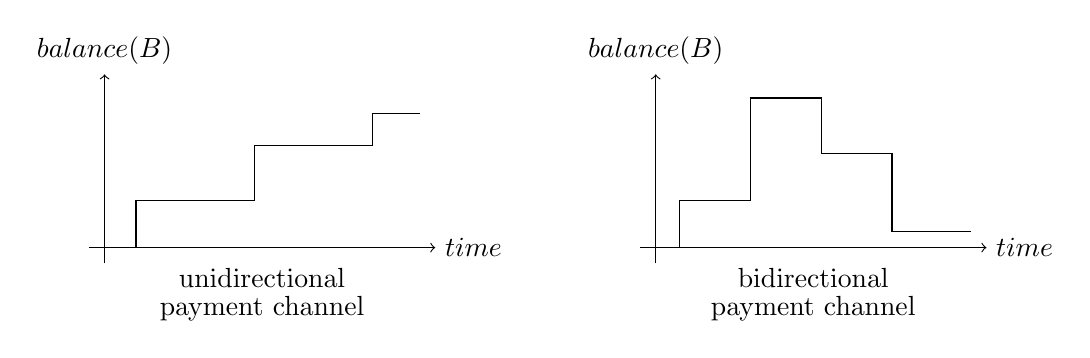
\begin{tikzpicture}[domain=0:2]
        \def\padding{0.1}
        \def\plotHeight{2}
        \def\plotWidth{4}
        \def\plotOffset{7}
        \def\textOffset{0.6}
        \foreach \i in {0,1} {
                \begin{scope}[shift={(\i*\plotOffset,0)}]
                    \draw[->] (-2*\padding,0) -- (\plotWidth+2*\padding,0) node[right] {$time$};
                    \draw[->] (0,-2*\padding) -- (0,\plotHeight+2*\padding) node[above] {$balance(B)$};

                    \ifnum\i=0
                        \path (0,-\textOffset) -- (\plotWidth,-\textOffset) node[midway] {\shortstack{unidirectional\\payment channel}};
                        \draw (0.4,0) -- (0.4,0.6) -- (1.4,0.6) -- (1.9,0.6) -- (1.9,1.3) -- (2.6,1.3) -- (3.4,1.3) -- (3.4,1.7) -- (4.0,1.7);
                    \else
                        \path (0,-\textOffset) -- (\plotWidth,-\textOffset) node[midway] {\shortstack{bidirectional\\payment channel}};

                        \draw (0.3,0) -- (0.3,0.6) -- (1.2,0.6) -- (1.2,1.9) -- (2.1,1.9) -- (2.1,1.2) -- (3.0,1.2) -- (3.0,0.2) -- (4.0,0.2);
                    \fi
                \end{scope}
            }
    \end{tikzpicture}
    \label{fig:channels}
    \caption{Node $A$ and $B$ have a payment channel. Whilst in case of unidirectional payment channels, $balance(B)$ is strictly increasing, the derivative of $balance(B)$ \textit{can} change sign if the channel is bidirectional.}
\end{figure}

\begin{figure}[H]
    \centering
    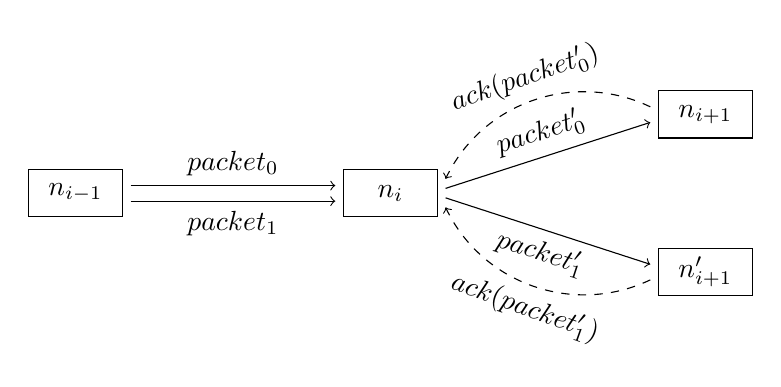
\begin{tikzpicture}
        \def\nodeOffset{4}
        \def\nodeYOffset{1}
        \def\nodeWidth{1.2}
        \def\nodeHeight{0.6}
        \def\padding{0.1}

        \foreach \xOffset\yOffset\name in{-\nodeOffset/0/$n_{i-1}$,0/0/$n_i$,\nodeOffset/\nodeYOffset/$n_{i+1}$,\nodeOffset/-\nodeYOffset/$n_{i+1}'$} {
                \draw[shift={(\xOffset,\yOffset)}] (0,0) rectangle (\nodeWidth,\nodeHeight) node[midway] {\name};
            }

        % Packets
        \draw[->,shift={(0,0.66*\nodeHeight)}] (-\nodeOffset+\nodeWidth+\padding,0) -- (-\padding,0) node[midway,above] {$packet_0$};
        \draw[->,shift={(0,0.33*\nodeHeight)}] (-\nodeOffset+\nodeWidth+\padding,0) -- (-\padding,0) node[midway,below] {$packet_1$};

        % Forwarded packets
        \draw[->] (\nodeWidth+\padding,0.6*\nodeHeight) -- (\nodeOffset-\padding,\nodeYOffset+0.33*\nodeHeight) node[midway,sloped,above] {$packet_0'$};
        \draw[->] (\nodeWidth+\padding,0.4*\nodeHeight) -- (\nodeOffset-\padding,-\nodeYOffset+0.66*\nodeHeight) node[midway,sloped,below] {$packet_1'$};

        % Acknowledgements
        \draw[->,dashed] (\nodeOffset-\padding,\nodeYOffset+0.66*\nodeHeight) to [bend right=45] node[above,sloped] {$ack(packet_0')$} (\nodeWidth+\padding,0.8*\nodeHeight);
        \draw[->,dashed] (\nodeOffset-\padding,-\nodeYOffset+0.33*\nodeHeight) to [bend left=45] node[below,sloped] {$ack(packet_1')$} (\nodeWidth+\padding,0.2*\nodeHeight);
    \end{tikzpicture}
    \caption{Node $n_{i-1}$ send packet $packet_0$, $packet_1$ to node $n_i$ which forwards them to node $n_{i+1}$ and node $n_{i+1}'$. Both nodes acknowledge the validity of $packet_0'$ and $packet_1'$ to node $n_i$.}
    \label{fig:sharedpaymentchannel}
\end{figure}

% Use data structure tickets

% Steady payments, expect continuous payments

% Entropy

% Continuous payments

\paragraph{Payment channels}

In traditional payment channels, two parties $A$ and $B$ lock some funds within a smart contract, make transactions off-chain and only commit the aggregation on-chain.



Thus, a payment channel is bidirectional, which means both $A$ and $B$ can send and receive transactions within the same payment channel. The HOPR protocol uses unidirectional payment channels to implement bidirectional payment channel behaviour, where one payment channel is created from $A$ to $B$ and another from $B$ to $A$. The payment channel creator is the sole owner of funds in the payment channel and the only one able to create \textbf{tickets}, encapsulated funds which are described in detail in Section \ref{sec:tickets}. A payment channel created from party $A$ to party $B$ is different from a payment channel created from party $B$ to party $A$.

$$A\rightarrow B \neq B\rightarrow A$$

\paragraph{Probabilistic payments}

This separation reflects the directional nature of packets flowing through the network. It also brings the advantage that each payment channel's logic is easier to verify.

\paragraph{Wrap Up}

\paragraph{Acknowledgements} are messages which allow every node to acknowledge the processing of a packet to the previous node. This acknowledgement ($ACK$) contains the cryptographic material needed to unlock the possible payout for the previous node. Note that an acknowledgement is always sent to the previous node, and using acknowledgments with vanilla payment channels results in accumulated incentives, where the latest acknowledgement contains all previous incentives plus the incentive for the most recent interaction, as explained below:

\begin{align}
    value (ACK_n) & =\sum_{i=1}^nfee_{packet_i},
\end{align}
where $n$ is the total number of mixnet packets transformed.

An issue arises when $B$ receives $ACK_n$ for $packet_n$ before sending $packet_{n-1}$. At this point $B$ would have no incentive to process $packet_{n-1}$ rather than $packet_{n}$. To avoid such false incentives, the HOPR protocol utilizes probabilistic payments. A \textit{ticket} can be either a win or a loss, determined based on some winning probability lower than 1. This means nodes are incentivized to continue relaying packets, as they do not know which tickets will result in a payout. From a node's perspective, each ticket has the same value until it is claimed; therefore, the HOPR protocol encourages nodes to claim tickets independently from each other.

\begin{align}
    value ( ACK_i ) & =value ( ACK_j ) \quad for \quad i,j\in \{1,\dots,n\}
\end{align}

If we assume constant costs, there is no added value in pretending packet loss or intentionally changing the order in which packets are processed. On the contrary, a node would reduce its potential payouts if it were to forward packets slowly or not at all.
